We compared the three proposed methods, GEA.1-3, as well as a pure generative model (GM) on a real object dataset. While it is hard to compare results across papers, GM arguably represents the state of the art for single-view dexterous grasping of novel objects, with a success rate of 77.8\% on a test-set of 45 novel objects seen from a single view\cite{kopicki2015ijrr}. In order to differentiate the algorithms, a new, more challenging, data set was created. This used 40 novel test objects (Figure~\ref{fig:real-objects}). Object-pose combinations were chosen to reduce the typical surface recovery. Some objects were employed in several poses, yielding 49 object-pose pairs. From the 40 objects, 35 belonged to object classes in the simulation dataset, while the remaining five did not. 

The difficulty of this new test-set was compared that of the previous one \cite{kopicki2015ijrr}. To make the two test-sets comparable the same set of five training grasps from \cite{kopicki2015ijrr} was used. The GM algorithm presented in \cite{kopicki2015ijrr} achieved a grasp success rate 77.8\% (35/45) on the original test set, but only 59.2\% (29/49) on the new test set. This is significant with a p-value of 0.043 under a one-tailed exact Fisher test. We therefore accept the hypothesis that the new data set of object-pose pairs is more challenging.

A pure generative model architecture (GM) and three generative-evaluative architectures (GEA.1-3) were evaluated using a paired trials methodology. Each was presented with the same object-pose combinations. Each architecture generated a ranked list of grasps, and the highest ranked grasp was executed. The highest-ranked grasp based on the predicted success probability of an evaluative network is performed on each scene. A grasp was deemed successful if, when lifted for five seconds, the object then remained stable in the hand for a further five seconds. The success rate for GM1 was 57.1\% and for the top-performing method based on GM1, GEA.1, it was 77.6\% (Table~\ref{tab:robot-results}). The success rate of the second baseline, GM2, is 81.6\%, while GEA.3 shows outperforms it with a success rate of 87.8\%. A two-tailed McNemar test, for the difference between success rates for paired comparison data, was performed. The difference between the two algorithms has a $p$-value of 0.0442, and so is statistically significant. A selection of grasps where the two methods performed differently are shown in Figure~\ref{fig:successfail}.

\begin{figure}
\begin{center}
  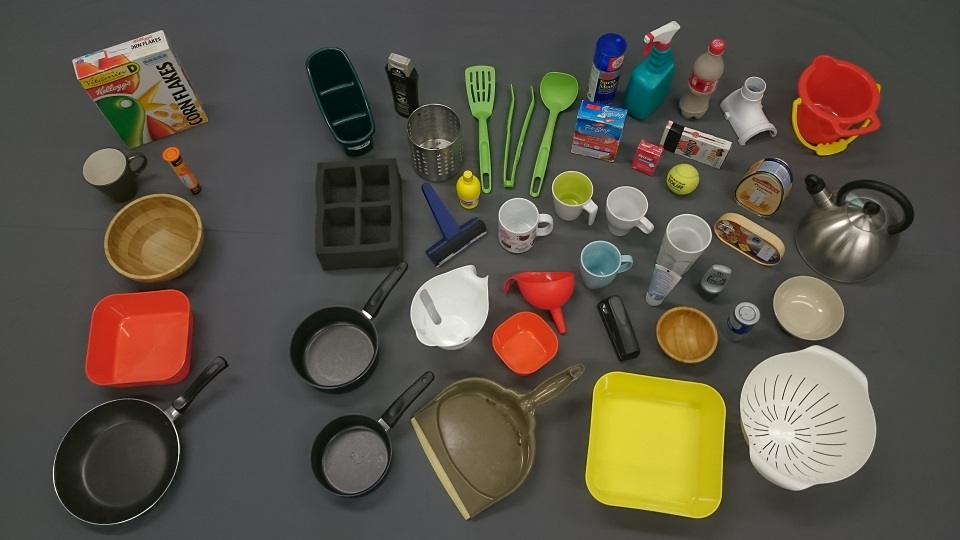
\includegraphics[width=0.9\linewidth]{images/objects.jpg}
  \end{center}
  \caption{The real objects. The training objects are on the left, testing objects are on the right.}
  \label{fig:real-objects}
\end{figure}

% OLD TABLE
%\begin{table}
%\begin{center}
%\caption{Results of the real robot paired comparison trial.}
%\begin{tabular}{|c|c|c|c|}  \hline 
%          &                & \multicolumn{2}{ c |}{ GM} \\ \hline
%          &                & \# succs & \# fails  \\  \hline
 %GEA  & \# succs &  23 &  15  \\
 %         & \# fails    &  5   &   6   \\ \hline
%\end{tabular}
%\end{center}
%\label{tab:robot-results}
%\end{table}

\begin{table}
\begin{center}
\caption{Results of the real robot paired comparison trial.}
\label{my-label}
\begin{tabular}{|cc|c|c|l}
\cline{1-4}
                                           &         & \multicolumn{2}{c|}{GM} &  \\ \cline{3-4}
                                           &         & \# succs    & \# fails    &  \\ \cline{1-4}
\multicolumn{1}{|c|}{\multirow{2}{*}{GEA}} & \# succs & 23         & 15         &  \\
\multicolumn{1}{|c|}{}                     & \# fails & 5          & 6          &  \\ \cline{1-4}
\end{tabular}
\end{center}
\label{tab:robot-results}
\end{table}


\begin{figure}
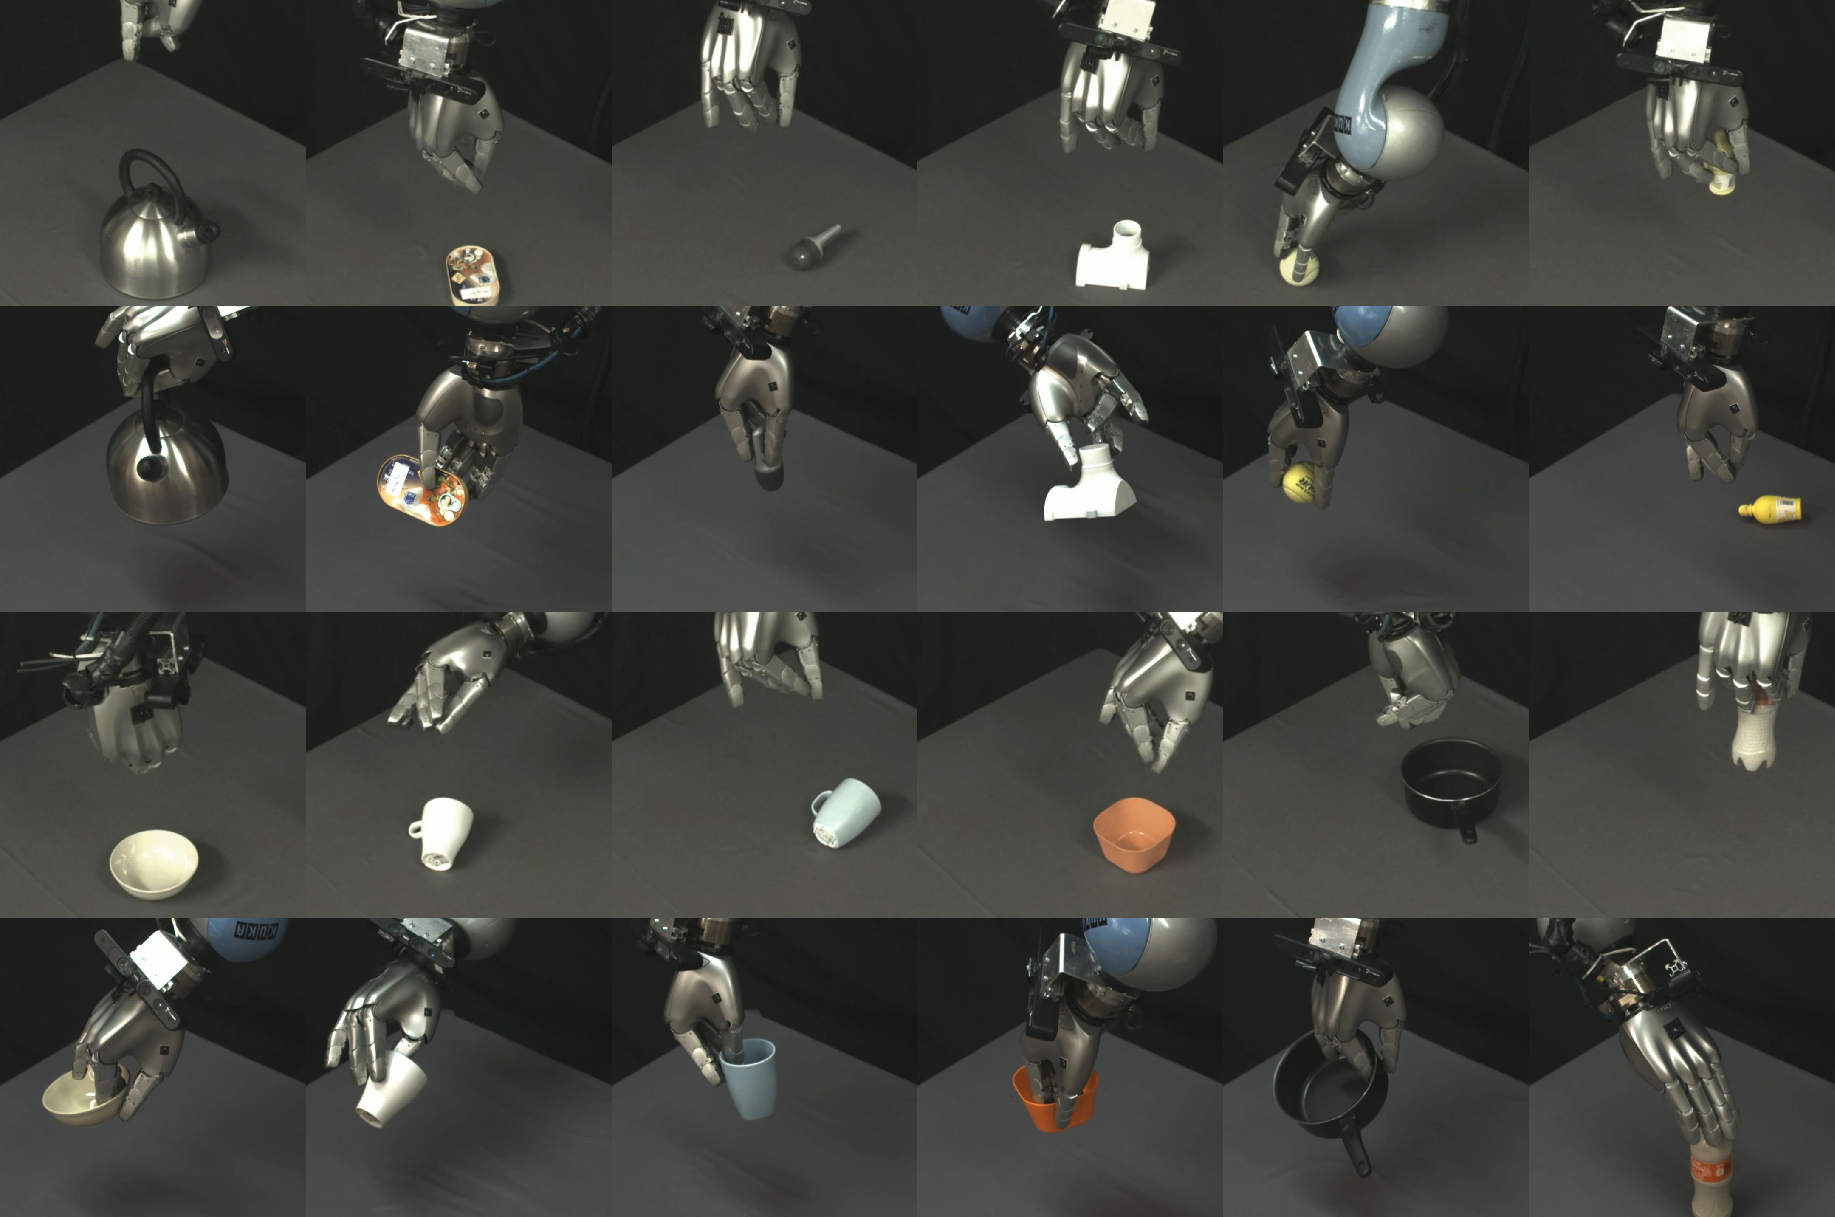
\includegraphics[width=\columnwidth]{images/successfailure.pdf}
\caption{Examples of grasps generated by the generative model (GM, $1^{st}$ and $3^{rd}$ row) and the generative-evaluative model (GEA, $2^{nd}$ and $4^{th}$ row) on paired trials. The first five columns show some of the 15 cases where the GEA model succeeds but GM fails. The far right-hand column shows 2 of the 5 converse cases. \label{fig:successfail}}
\end{figure}

%Training parameters for network. Training of example grasps for learning from demonstration. Creation of real test data set. Paired comparisons methodology with vanilla LFD algorithm (pose + object + camera view).
%
%The actual grasping tests have been performed on the real robot. 